\documentclass[12pt,fleqn,a4paper,oneside]{LegrandOrangeBook}
\addbibresource{sample.bib} % Bibliography file
\definecolor{ocre}{RGB}{103, 61, 76}
\chapterimage{orange1.jpg} 
\chapterspaceabove{6.5cm}
\chapterspacebelow{6.75cm} 
%\begin{theorem}[Name of the theorem]
%\begin{exercise}
%\begin{example}[Example name]
%\begin{definition}[Definition name]
%\begin{corollary}[Corollary name]
%\begin{remark}
%\begin{proposition}[Proposition name]
%\begin{problem}
%\begin{vocabulary}[Word]
%\begin{notation}
%----------------------------------------------------------------------------------------
\begin{document}
%----------------------------------------------------------------------------------------
%----------------------------------------------------------------------------------------
%Lineas
%----------------------------------------------------------------------------------------
\section{Líneas desacoplada y ondas estacionarias}\index{Líneas desacoplada y ondas estacionarias}
Seguiremos con el estudio con $\alpha=0$ (sin pérdidas) y altas frecuencias.
%----------------------------------------------------------------------------------------
%Internetworking
%----------------------------------------------------------------------------------------
\section{Métodos para control de la congestión}
\begin{figure}[H]
\centering
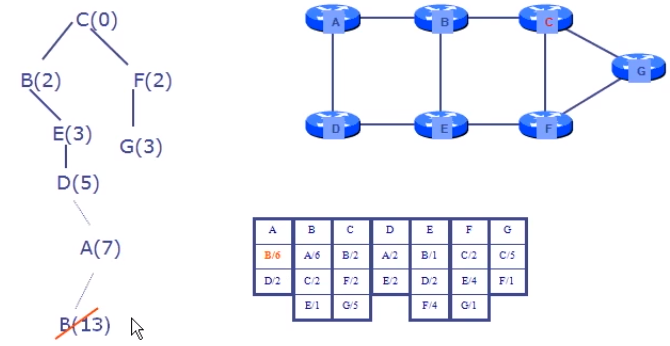
\includegraphics[width=0.8\linewidth]{IN1/IN75.png}
\caption{Escalas de tiempo de los métodos para el control de la congestión.}
\end{figure}
\subsection{Enrutamiento consiente de tráfico}
El objetivo es desviar el tráfico de los puntos más activos hacia otros, esto esta en desuso debido a su oscilación
\begin{center}
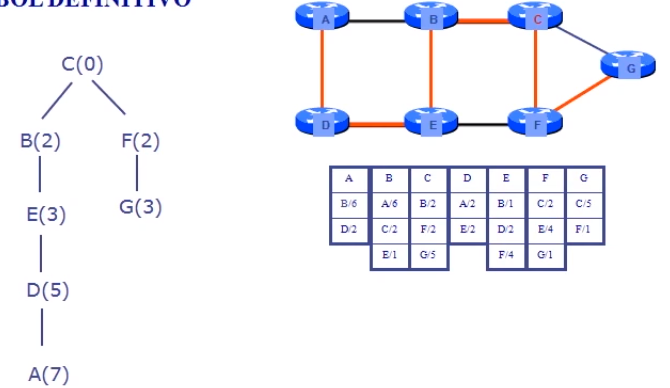
\includegraphics[width=0.8\linewidth]{IN1/IN76.png}
\end{center}
Sean dos sistemas autónomos como la image, los enlaces entre ambos sistemas son CF y EI, al congestionarse CF se enrutará los paquetes hacia EI para despejar CF. Pero luego de este proceso EI estará congestionado y verá EI como una ruta optima. El sistema de enrutamiento será \textbf{oscilatorio}.
\subsection{Regulación de tráfico}
\begin{figure}[H]
\centering
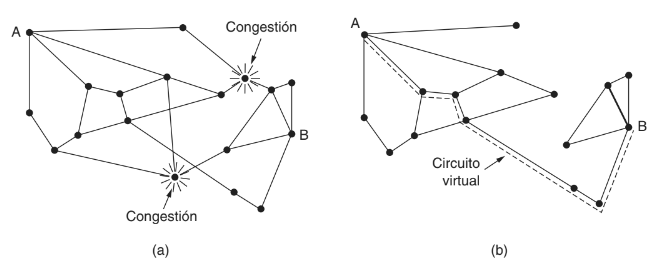
\includegraphics[width=\linewidth]{IN1/IN77.png}
\caption{(a) Una red congestionada. (b) La parte de la red que no esta congestionada.}
\label{fig:regulacion trafico}
\end{figure}
En la figura \ref{fig:regulacion trafico}.a se muestra la red con dos puntos de congestión, lo que haremos es eliminar esos puntos de congestión y calculando una nueva ruta virtual evitando los puntos de congestión. El problema puede ser que esta desviación tome un poco más de tiempo. Al existir una congestión, el router congestionado devuelve un trama al azar y envía un \textbf{paquete regulador} con un bit de encabezado al emisor para que no generé más paquetes y se reduzca el tráfico. Esto no es equitativo pues los emisor más rápidos tendrán más paquetes congestionados que lo emisores lentos.
\subsubsection{ECN}
ENC o notificación explicita de congestión, funciona similar al \textbf{paquete regulador}, en vez de crear un datagrama que vuelva al emisor, se configura dos bits para que cuando lleguen al receptor este se enteré en donde hubo una congestión y este mandará un mensaje al emisor directo para que tome las medidas.
%%22:27l
%----------------------------------------------------------------------------------------
%Microprocesadores
%----------------------------------------------------------------------------------------

%----------------------------------------------------------------------------------------
%Mantenimiento
%----------------------------------------------------------------------------------------

%----------------------------------------------------------------------------------------
\end{document}
%----------------------------------------------------------------------------------------
